\begin{blocksection}
\question 
In this question, you will be analyzing the virtual memory system of a single-­processor, single-­core computer with 4 KiB pages, 1 MiB virtual address space and 1 GiB physical address space. 
The computer has a single TLB that can store 4 entries. You may assume that the TLB is fully ­associative with an LRU replacement policy, and each TLB entry is as depicted below.

TLB Entry \\
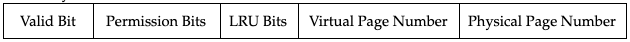
\includegraphics[width=\textwidth]{virtualmemory/taggedtlbentry}

\begin{parts}
\part
Given a virtual address, how many bits are used for the Virtual Page Number and Offset?

\begin{solution}[0.5in]
VPN: 8, Offset: 12.
There is 1 MiB of virtual memory so each virtual address is  $\log_2(2^{20})$ = 20 bits in total. 
We know that each page is 4 KiB, so the offset is $\log_2(2^{12})$ = 12 bits. This leaves 8 bits for the virtual page number.
\end{solution}

\part
Given a physical address, how many bits are used for the Physical Page Number and Offset?

\begin{solution}[0.5in]
PPN: 18, Offset: 12
The offset will remain 12 bits, as the page size is constant. Physical memory is 1 GiB, so, as physical addresses are
$\log_2(2^{30})$ = 30 bits wide, we have 18 bits for the physical page number
\end{solution}
\end{parts}

\end{blocksection}